\documentclass{llncs}
\usepackage[utf8]{inputenc}
\usepackage[T1]{fontenc}
\usepackage{graphicx}

\graphicspath{{resources/}}

\begin{document}

\title{ConfiguraFácil}
\author{Alexandre Pinho, Joel Gama, Tiago Pinheiro}

\institute{
University of Minho, Department of  Informatics, 4710-057 Braga, Portugal, \\
\email{a82441@alunos.uminho.pt},\email{a82202@alunos.uminho.pt},\email{a82491@alunos.uminho.pt}
}

\maketitle

\clearpage

\section{Introdução}

Este projeto surge no âmbito da UC de Desenvolvimento de Sistemas de Software, que faz parte do Mestrado Integrado em Engenharia Informática, da Universidade do Minho.

Foi-nos proposto desenvolver um sistema que tem dois principais usos: a encomenda de um carro segundo uma configuração escolhida pelo cliente; e a utilização do software no chão da fábrica, que inclúi o registo da chegada de componentes e a gestão da fila de espera da produção dos carros. 

As seguintes secções descrevem o processo de desenvolvimento do projeto seguido pelo grupo, as escolhas de design da arquitetura feitas pelo grupo, e o resultado final obtido. Por fim, é feita uma análise crítica ao trabalho desenvolvido.

\clearpage
\section{Processo de desenvolvimento}

%parte introdutória

\subsection{Modelação do domínio}

O primeiro passo no processo de desenvolvimento consiste na modelação do domínio do problema. Representam-se gráficamente as entidades do problema e os relacionamentos entre si. Esta fase é a melhor ocasião para esclarecer quaisquer dúvidas ou inconsistências com o cliente. No fim, já é possível começar a identificar os principais conceitos e funcionalidades da aplicação, a ser especificados posteriormente.

\begin{figure}
\begin{center}
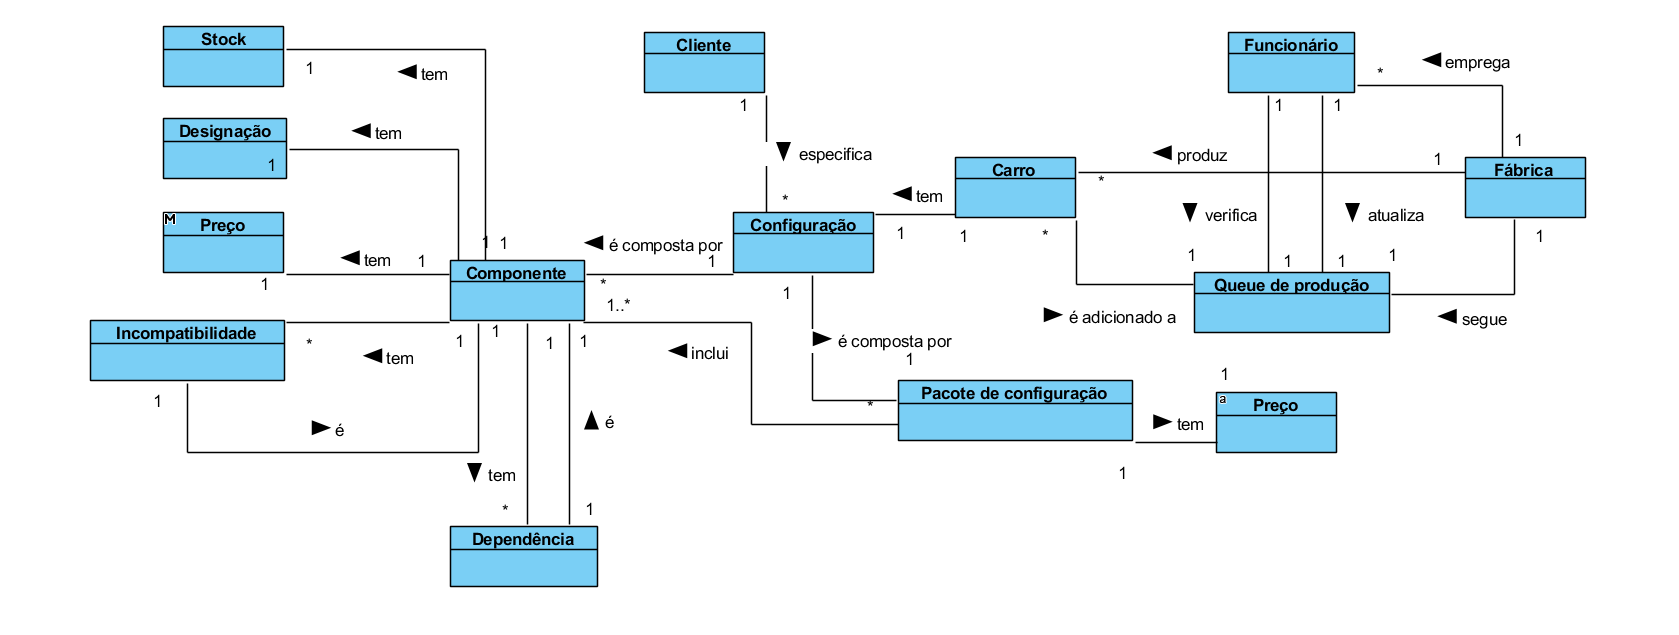
\includegraphics[scale=0.25]{modelo_de_dominio.png} 
\end{center}
\caption{\label{fig:modelo_dominio}Modelo de domínio}
\end{figure} 


Como podemos visualizar na figura \ref{fig:modelo_dominio}, o grupo identificou, para além das características básicas de um componente e entidades auxiliares, várias entidades principais: o componente, o pacote de configuração, a configuração, o cliente, o carro, e a queue de producao. 

\subsection{Modelação dos requesitos funcionais}

Com a modelação do domínio do problema feita, é necessário identificar os requesitos funcionais da aplicação, ou seja, os diferentes casos de uso (Use Cases) da aplicação. Esta modelação é importante por várias razões: para além de identificar o que a aplicação faz em concreto e facilitar o teste da aplicação, também serve para esclarecer, tanto para o programador como para o cliente, o que a aplicação não faz.

\begin{figure}
\begin{center}
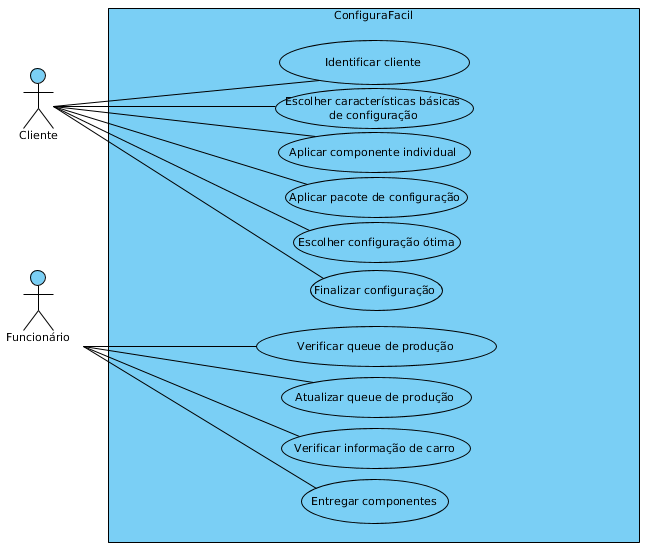
\includegraphics[scale=0.40]{diagrama_use_cases.png} 
\end{center}
\caption{\label{fig:diagrama_use_cases}Diagrama de Use Cases}
\end{figure} 

Na aplicação a desenvolver neste projeto foram identificados dois atores (cliente e funcionário) e dez Use Cases. O diagrama de Use Cases da figura \ref{fig:diagrama_use_cases} representa gráficamente esta informação.

\subsection{Especificação dos Use Cases}

\begin{figure}
\begin{center}
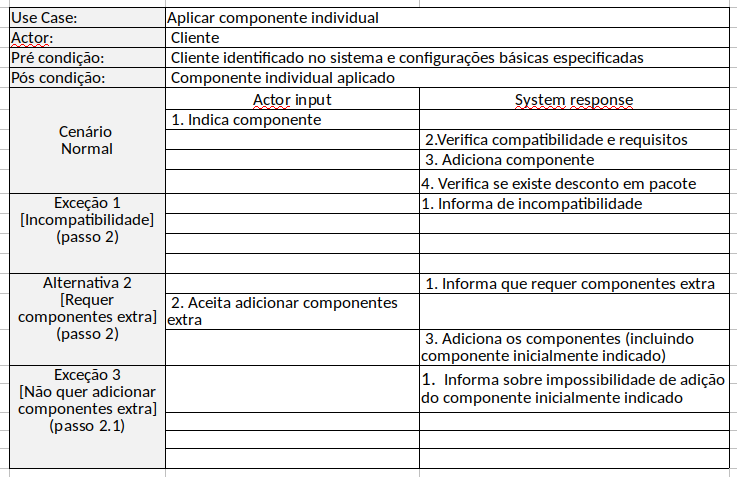
\includegraphics[scale=0.40]{aplicar_componente_tabular.png} 
\end{center}
\caption{\label{fig:notacao_tabular}Especificação do Use Case "Aplicar componente individual" em notação tabular }
\end{figure} 

Depois de identificados os Use Cases é feita a sua especificação, representando em notação tabular a interação entre o ator e o sistema, como por exemplo na figura \ref{fig:notacao_tabular}.

\subsection{Conceção da interface}

De forma a consultar com o cliente e ter o seu feedback, foi desenvolvido na fase inicial do projeto um protótipo de baixa fidelidade do aspeto da interface, e foi desenhado um diagrama de máquinas de estado a descrever o comportamento da interface. Embora o desenho da interface tenha mudado ao longo do desenvolvimento da aplicação, as ideias básicas são as mesmas, não sendo o produto final fundamentalmente diferente.

\subsection{Modelação comportamental}

\clearpage
\section{Conceção da solução} % título de secção melhor?




\clearpage
\section{Conclusão}

\end{document}
